
Il data-set considerato � pubblicato su \url{https://rebrickable.com/downloads/}. La tabelle sono state create con il tool HeidiSQL a partire dal diagramma relazionale a disposizione. I dati, aggiornati ogni giorno, si possono caricare a partire dai file csv di ogni tabella con la funzionalit� di import a partire da file csv.

Non tutte le tabelle della base dati sono servite per le funzionalit� implementate: quelle utilizzate sono schematizzate nella figura \ref{FIG:base_dati}. In grigio � evidenziata una tabella non presente nella base dati pubblicata e introdotta per modellare il magazzino del collezionista.
Il pezzo � univocamente identificato attraverso un codice, il colore e il materiale. Ogni set � composto da uno o pi� pezzi e appartiene a una serie.
Una breve descrizione di ciascuna tabella � indicata nella tabella \ref{TAB:descrizione_base_dati}

\newpage
\vspace{0.5cm} 
\begin{figure}[htbp]
\centering
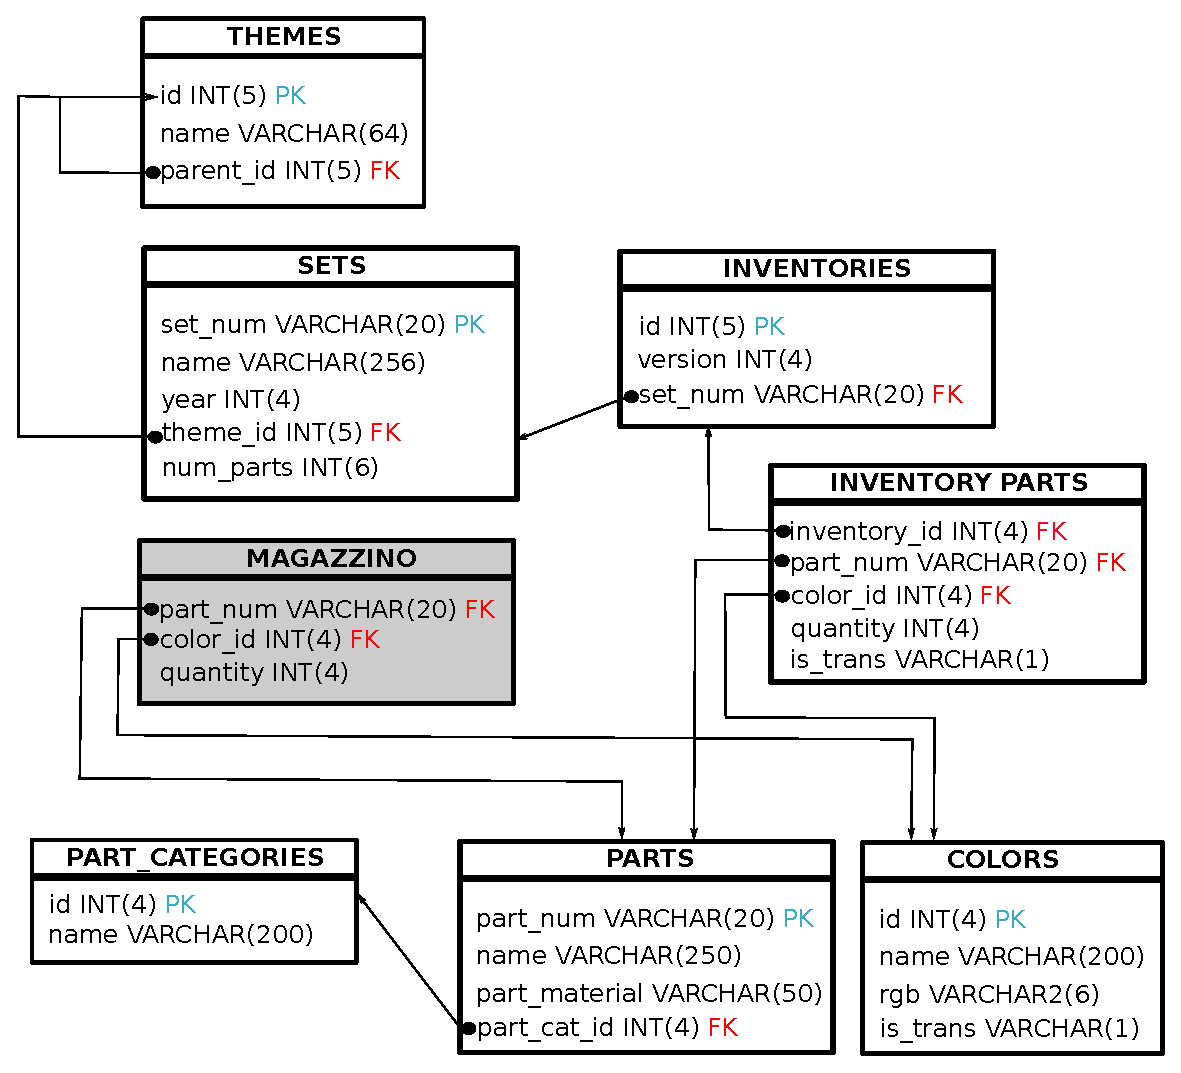
\includegraphics[scale=0.65]{data_set/base_dati.eps}
\vspace{6.5cm} \caption{Base dati considerata dall'applicazione di gestione/analisi magazzino Lego}
\label{FIG:base_dati}
\end{figure}
\vspace{0.5cm} 

\newpage


\begin{table}[htbp]
\begin{center}
\begin{tabular}{||p{0.23\linewidth}|p{0.18\linewidth}|p{0.1\linewidth}|p{0.15\linewidth}|p{0.25\linewidth}||}
\hline
{\bfseries tabella} & scopo & numero record & chiave primaria PK & chiavi esterne FK\\
\hline
\hline
\texttt{themes} & elenco di tutte le serie in commercio & circa 500 & campo id & il campo parent\_id assume solo valori contenuti nel campo id. Se valorizzato, indica che la serie un filone di un'altra principale \\
\hline
\texttt{sets} & elenco di tutti i set in commercio & circa 15000 & campo \texttt{set\_num} & il campo \texttt{theme\_id} assume solo valori contenuti nel campo id della tabella theme. Ogni set � quindi associato a una serie. \\
\hline
\texttt{parts} & elenco di tutti i pezzi in commercio & circa 35000 & campo \texttt{part\_num} & \\
\hline
\texttt{colors} & elenco di tutti i colori dei pezzi & circa 200 & campo \texttt{id} & \\
\hline
\texttt{inventories} e \texttt{inventory\_parts} & relazionano i set e i pezzi che lo compongono & circa 750000 & & campi \texttt{part\_num}, \texttt{color\_id} e \texttt{inventory\_id}\\
\hline
\texttt{colors} & elenco di tutti i colori dei pezzi & circa 200 & id & \\
\hline
\texttt{magazzino} & contiene i pezzi a disposizione del collezionista. In continuo aggiornamento & & & campi \texttt{part\_num} e \texttt{color\_id}\\

\hline
\hline
\end{tabular}
\caption {\label{TAB:descrizione_base_dati}  Descrizione e caratteristiche delle tabelle utilizzate}
\end{center}
\end{table}
\vspace{0.5cm}
